% !TeX spellcheck = de_DE
\documentclass[10pt, a4paper]{amsart}
\usepackage[utf8x]{inputenc}
\usepackage{polyglossia}
\setdefaultlanguage{ngerman}
\usepackage{enumitem}
\usepackage{caption}
\captionsetup[figure]{name=Abbildung}
\usepackage{tkz-euclide}
\usepackage{amsmath, amsfonts, amssymb}
\usepackage{amsthm, thmtools}
\declaretheorem[name=Aufgabe, thmbox = L]{aufgabe}
\declaretheorem[name=Lemma]{lemma}
\counterwithin*{lemma}{aufgabe}
\counterwithin*{equation}{aufgabe}
\newcommand{\aufgabelabelname}{\theaufgabe . Aufgabe}
\renewcommand\qedsymbol{$\blacksquare$}

\usepackage{physics}
\usepackage{fancyhdr}
\pagestyle{fancy}
\fancyheadoffset{0cm} 
\usepackage[
  a4paper,
  right=6cm,
  footskip=3em,
  twoside=false,
  lmargin=1.4cm,
  xetex
]{geometry}
\usepackage{unicode-math}
\listfiles
\makeatletter
\renewenvironment{proof}[1][\proofname]{\par
\pushQED{\qed}%
\normalfont \topsep6\p@\@plus6\p@\relax
\trivlist
\item\relax
{\bfseries#1}\hspace\labelsep\ignorespaces
}{%
\popQED\endtrivlist\@endpefalse
}
\newenvironment{proof_thm}[1]{
\begin{proof}[\proofname~(#1)]}{\end{proof}}
\makeatother

\chead{
	\fontsize{9}{7}\large\aufgabelabelname
}
\rhead{
	\fontsize{9}{7}Valentin Herrmann}

%hyperref must be the last package in the preamble
\usepackage{hyperref}
\hypersetup{
	bookmarks=true,
	unicode=true,
	pdfborder={0 0 0},
	pdfstartview={FitH},
	pagebackref=true,
	colorlinks=true,
	urlcolor=blue,
	linkcolor=black,
	linktoc=all
}
\renewcommand{\figureautorefname}{Abbildung}

\begin{document}
\thispagestyle{fancy}
\begin{aufgabe}
  Leo und Smilla finden 2020 Goldnuggets mit den Massen 1, 2, ..., 2020 Gramm,
  die sie nach folgender Regel auf eine rote und eine blaue Schatztruhe
  verteilen:
  
  Zuerst wählt Leo eine der Schatztruhen und nennt Smilla die Farbe der Truhe.
  Anschließend wählt Smilla eines der noch nicht verteilten Nuggets und legt es
  in diese Truhe. Dies wiederholen sie, bis alle Nuggets verteilt sind. Danach
  wählt Smilla eine der beiden Schatztruhen und bekommt alle Nuggets in dieser
  Truhe.

  Wie viel Gramm Gold kann Smilla auf diese Weise mindestens für sich
  garantieren?
\end{aufgabe}
\begin{lemma}\label{sec1:Zahlensumme}
  Es gilt für alle $n∈ℕ^*$:
  \[ \sum^{n}_{k=1}k=\dfrac{n(n+1)}{2}\]
\end{lemma}
\begin{lemma}
  \label{sec1:zahlengruppen}
  Jeder Abschnitt der natürlichen Zahlen, welcher mit 1 beginnt und mit einer
  Zahl $n=4k+3$, $k∈ℕ_0$ aufhört kann in zwei gleich große Gruppen geteilt
  werden.
\end{lemma}
\begin{proof}
  Für einen einfacher lesbaren Beweis werden die Nuggets jeweils nach ihrer
  Masse benannt. Nugget $1234$ steht also für das Nugget mit der Masse $1234$g.
  
  Zuerst wird die Obergrenze für Smillas maximalen Schatz bestimmt. Für die
  Situation vor der Vergabe des letzten Nuggets $n_{2020}$ in die beiden Truhen
  mit Gewicht $r_{2019}$ und $b_{2019}$ gilt unter Anwendung
  von~\autoref{sec1:Zahlensumme}:
  \begin{equation}\label{sec1:equation1}
    r_{2019}+b_{2019}=\sum_{k=1}^{2020}\left(k\right)-n_{2020}=\dfrac{2020\cdot2021}{2}-n_{2020}
  \end{equation}
  Da Smilla sich am Schluss ihre Truhe aussuchen darf und daher die schwerere
  Truhe bekommt, wodurch Leo die Leichter bekommt, wird Leo versuchen die Truhen
  so gleichmäßig wie möglich zu füllen. Also wird Leo logischerweise die
  leichtere Truhe für das letzte Nugget wählen, sodass der letztendliche
  Gewichtsunterschied möglichst klein ist. Sind die Truhen gleich schwer so ist
  es unerheblich für Leo, welche Truhe er wählt. Angenommen die rote Truhe mit
  Gewicht $r_{2019}$ ist leichter oder gleich schwer wie die Blaue vor der
  Vergabe des letzten Nuggets (Die Farben sind austauschbar), dann wird Leo die
  rote Truhe wählen und Smilla wird das letzte Nugget $n_{2020}$ in diese Truhe
  legen. Daraus folgt mit~\eqref{sec1:equation1}:
  \begin{equation}\label{sec1:equation2}
    r_{2020}=r_{2019}+n_{2020}=(1010\cdot2021-b_{2019}-n_{2020})+n_{2020}=1010\cdot2021-b_{2019}
  \end{equation}
  Also hat $r_{2020}$ den maximalen Wert, wenn $b_{2019}$ minimal ist. Da
  $b_{2019}$ größer gleich $r_{2019}$ sein muss, ist der minimale Wert von
  $b_{2019}$ also $r_{2019}$. Im Idealfall folgt daher
  mit~\eqref{sec1:equation1}:
  \begin{equation}\label{sec1:equation3}
    \begin{split}
      2b_{2019} &= 2r_{2019} =1010\cdot2021-n_{2020}\\
      \Rightarrow b_{2019} &= r_{2019}=5050\cdot2021-\dfrac{n_{2020}}{2}
    \end{split}
  \end{equation}
  Wird~\eqref{sec1:equation3} in \eqref{sec1:equation2} eingesetzt:
  \begin{equation*}
    r_{2020}=5050\cdot2021+\dfrac{n_{2020}}{2}
  \end{equation*}
  Im Idealfall für Smilla ist $n_{2020}$ maximal groß und hat daher den Wert
  2020. Damit gilt für die Obergrenze $r_{2020}$:
  \begin{equation*}
    r_{2020}=5050\cdot2021+1010
  \end{equation*}
  Nun stellt sich die Frage, ob Smilla diese Obergrenze überhaupt erreichen
  kann. Eine Strategie für Smilla um mindestens die Obergrenze zu erreichen ist Folgende:\\

  Smilla trennt alle Nuggets bis auf $2020$ nach in zwei gleich schwere Gruppen.
  Das ist möglich, da $2019$ gleich $4\cdot504 + 3$ ist,
  weshalb~\autoref{sec1:zahlengruppen} anwendbar ist. Die Gruppen entsprechen
  dabei den Truhen. Wählt nun Leo eine Truhe aus, so legt Smilla ein Nugget aus
  der entsprechenden Gruppe hinein. Wählt Leo irgendwann eine Truhe aus, in
  welcher schon alle Nuggets der entsprechenden Gruppe sind, so legt Smilla das
  Nugget 2020 in diese Truhe, womit die Obergrenze erreicht ist. erhalten.
\end{proof}
\begin{proof_thm}{\autoref{sec1:Zahlensumme}}
  \begin{align*}
    \sum^{n}_{k=1}k&=\dfrac{1}{2}\cdot\left( \sum^{n}_{k=1}k +
                     \sum^{n}_{k=1}(n+1-k)\right) = \dfrac{1}{2}\cdot\sum^{n}_{k=1}(k+(n+1-k))\\
                   &=\dfrac{1}{2}\cdot\sum^{n}_{k=1}(n+1) = \dfrac{n(n+1)}{2}
  \end{align*}
\end{proof_thm}
\begin{proof_thm}{\autoref{sec1:zahlengruppen}}
  Die Zahlenreihe wird um Null erweitert, sodass die Reihe aus insgesamt
  $n+1=4(k+1)$ Zahlen besteht. Nun wird die Zahlenfolge in der Mitte „gefaltet“.
  Die kleinste Zahl wird mit der Größten gepaart, die zweit Kleinste mit der
  zweit Größten, etc. So enstehen $\frac{4(k+1)}{2}=2(k+1)$ Paare, jeweils mit
  einer Summe von $(j)+(n-j) = n+1$. Da die Paare alle gleich groß sind und eine
  gerade Anzahl haben, können sie in zwei gleich große Gruppen unterteilt
  werden. Dabei kann nun die Null wieder entfernt werden, schließlich verändert
  sie die Summen der Gruppen nicht.
\end{proof_thm}

\newpage
\begin{aufgabe}
  Beweise: Es gibt keine rationalen Zahlen $x$, $y$, $z$ mit $x + y + z = 0$ und
  $x + y + z = 100$.
\end{aufgabe}
\begin{lemma}\label{sec2:rational1}
  Jeder Quotient $\frac{a}{b}$ zweier rationaler Zahlen $a,b∈ℚ\backslash\{0\}$
  ist rational definiert.
\end{lemma}
\begin{lemma}\label{sec2:rational2}
  Jedes Produkt $ ab $ einer rationalen Zahl $a$ ungleich Null und einer
  irrationalen Zahl $b$ ist immer eine irrationale Zahl.
\end{lemma}
\begin{proof}
  Zuerst wird $x+y+z = 0 \Rightarrow z = -(x+y)$ in $x^2+y^2+z^2 = 100$
  eingesetzt. Also gilt:
  \begin{equation}
    \label{eq:1}
    x^2+y^2+(-(x+y))^2 = 100 \Rightarrow x^2+xy+y^2=50
  \end{equation}
  Hieraus folgt direkt, dass $x$ und $y$ nicht gleich Null sein können. Sind sie
  beide Null, so gilt: $0^2+0\cdot0+0^2=0\neq50$. Ist nur eine der Variablen
  Null so gilt: $0^2+0\cdot a+a^2=a^2=50\Rightarrow a = \pm5\sqrt{2}$. a kann
  dabei durch x oder y substituiert werden. Da $\sqrt{2}$ irrational ist, ist
  nach~\autoref{sec2:rational1} auch dieser Fall nicht möglich, sonst wäre $a$
  schließlich irrational.

  Durch Teilen von~\eqref{eq:1} durch $x^2$ entsteht
  $(\frac{y}{x})^2+\frac{y}{x}+1=\frac{50}{x^2}$. Das Teilen durch $x^2$ ist
  erlaubt, da $x$ nicht Null sein kann.
  
  Aus~\autoref{sec2:rational2} folgt, dass $q=\frac{y}{x}$ als eine gekürzte
  rationale Zahl $\frac{m_q}{n_q}$ mit $m_q,n_q\in\mathbb{Z}\backslash\{0\}$,
  wobei $m_q$ und $n_q$ teilerfremd sind, beschreibbar sein muss. Auch $x$ muss
  als rationale Zahl $\dfrac{m_x}{n_x}$, mit
  $m_x,n_q\in\mathbb{Z}\backslash\{0\}$, wobei $m_x$ und $n_x$ teilerfremd sind.
  Also kann die Gleichung umgeschrieben werden:
  \begin{equation}
    \label{eq:2}
    \begin{split}
      \left(\dfrac{m_q}{n_q}\right)^2+\dfrac{m_q}{n_q}+1&=\dfrac{50}{\left(\frac{m_x}{n_x}\right)^2}=2\dfrac{5n_x^2}{m_x^2}\\
      \Rightarrow \dfrac{m_q^2+m_q\cdot n_q +
        n_q^2}{2}&=\dfrac{5^2n_x^2n_q^2}{m_x^2}=\left( \dfrac{5n_xn_q}{m_q}
      \right)
    \end{split}
  \end{equation}
  Da die rechte Seite von~\eqref{eq:2} das Quadrat einer rationalen Zahl ist,
  gilt dies auch für $\frac{m_q^2+m_q\cdot n_q + n_q^2}{2}$. Da Qudrate von
  rationalen Zahlen immer eine gerade Anzahl ihrer Primfaktoren haben, muss das
  auch für $2$ gelten. Daher wird zwischen drei Fällen unterschieden:
  \begin{itemize}[itemsep=2ex]
  \item Sind $m_q$ und $n_q$ beide ungerade:
    \[m_q^2+m_qn_q+n_q^2\equiv1^2+1\cdot1+1^2\equiv1\pmod{2}\] Also ist in
    diesem Fall der Zähler ungerade. Damit der Nenner der linken Seite
    von~\eqref{eq:2} die ungerade Anzahl $2^{-1}$vom Primfaktor 2, womit die
    linke Seite kein Qudrat einer rationalen Zahl sein kann. Es gibt einen
    Widerspruch.
  \item Ist $m_q$ gerade und $n_q$ ungerade:
    \[m_q^2+m_qn_q+n_q^2\equiv0^2+0\cdot1+1^2\equiv1\pmod{2}\] Auch hier ist
    wird der Zähler ungerade, womit gleiches wie im vorherigen Fall gilt.
  \item Da der Zähler symmetrisch in Rücksicht auf $m_q$ und $n_q$ ist, gilt
    wenn $m_q$ ungerade und $n_q$ gerade ist, gleiches wie im vorher gehenden
    Fall.
  \item Es können nicht beide Variablen gerade sein, da sie nach Definition teilerfremd sein
    müssen.
  \end{itemize}
  Damit kann $\frac{y}{x}$ keine rationale Zahl sein, wenn $x$ eine rationale
  Zahl ist. Doch gleichzeitig folgt aus~\autoref{sec2:rational1}, dass
  $\frac{y}{x}$ eine rationale Zahl sein muss, wenn $x$ und $y$ rational sind.
  Also können $x$ und $y$ nicht gleichzeitig rational sein.
\end{proof}
\begin{proof_thm}{\autoref{sec2:rational1}}
  Wird $a$ durch $\frac{m_a}{n_a}$ und $b$ durch $\frac{m_b}{n_b}$ beschrieben,
  wobei $m_a,n_a,m_b,n_b\inℕ^*$ gilt, so kann der Quotient $\frac{a}{b}$ als
  $\frac{\frac{m_a}{n_a}}{\frac{m_b}{n_b}}=\frac{m_a\cdot n_b}{m_b\cdot n_a}$
  geschrieben werden. Da $m_a\cdot n_b$ und $m_b\cdot n_a$ ganze Zahlen ungleich
  Null sind, muss der Quotient rational sein.
\end{proof_thm}
\begin{proof_thm}{\autoref{sec2:rational2}}
  Beweis durch Widerspruch: Angenommen das Produkt $c$ ist eine rationale Zahl:
  \begin{equation*}
    ab=c \Rightarrow b =\frac{c}{a}
  \end{equation*}
  Die rechte Seite muss nach~\autoref{sec2:rational1} rational sein, also darf
  $b$ nicht irrational sein.
\end{proof_thm}

\newpage
\begin{aufgabe}
  Zwei Geraden $m$ und $n$ schneiden sich in genau einem Punkt $P$. Ein Punkt
  $M$ bewegt sich auf m mit konstanter Geschwindigkeit, ein weiterer Punkt $N$
  bewegt sich auf $n$ mit derselben Geschwindigkeit; dabei passieren sie beide
  den Punkt $P$, aber nicht gleichzeitig.
 
  Beweise: Es gibt einen festen, von $P$ verschiedenen Punkt $Q$ so, dass die
  Punkte
  $P$, $Q$, $M$ und $N$ zu jedem Zeitpunkt auf einem gemeinsamen Kreis liegen.\\
\end{aufgabe}
\begin{lemma}\label{sec3:lemma1}
  Für alle festen, veschiedenen Punkte $P$ und $Q$, existiert eine Gerade $g$, sodass
  genau dann wenn der Mittelpunkt $M$ eines Kreises $k$ auf $g$ und $P$ auf $k$
  liegt, auch $Q$ auf dem Kreis liegt.
\end{lemma}
\begin{lemma}\label{sec3:lemma2}
  Sind in einem Dreieck zwei Höhen gleich, so muss das Dreieck gleichschenklig
  sein. Dabei sind die Seiten auf welchen die Höhen stehen die Schenkel des
  Dreiecks.
\end{lemma}
\begin{proof}
  Zuerst wird die Position des Umkreismittelpunkts $U$ von $PMN$ in Abhängigkeit
  der Zeit $t$ bestimmt. Denn nur exakt dann wenn alle $U$ auf einer Geraden
  liegen, existiert nach~\autoref{sec3:lemma1} ein weiterer Punkt außer $P$,
  welcher für alle verschiedenen $U$ auf dem Kreis liegt.

  Um das zu beweisen werden nun alle $U_t$
  mit einem $U_0$ verglichen. Der Umkreismittelpunkt eines Dreiecks wird durch
  den Schnittpunkt der Mittelsenkrechten der Dreiecksseiten bestimmt. Zwei
  Mittelsenkrechten reichen dabei aus:
  
  \begin{figure}[h]
    \centering
      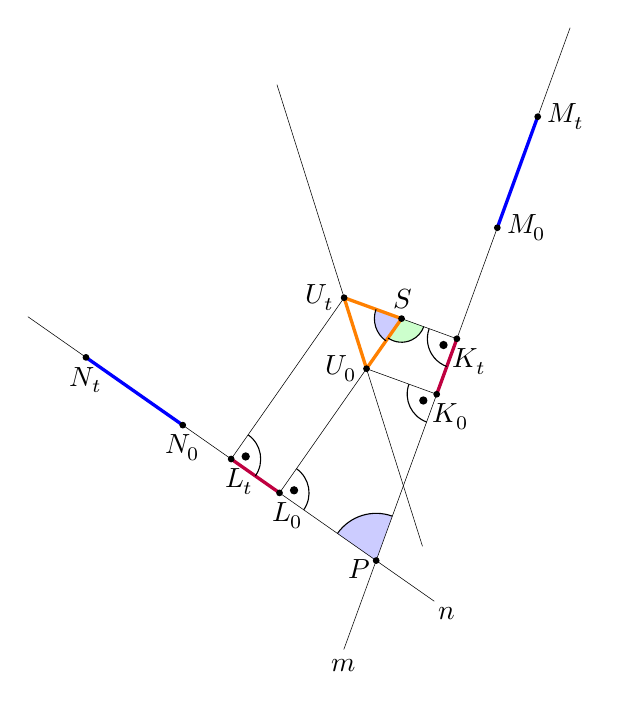
\begin{tikzpicture}[rotate=70,scale=1.5]
        % \tkzSetUpLine[add=.5 and .5]%
        \tkzSetUpPoint[fill=black]%
    
        \def\vara{75} \def\varx{1}%
    
        \tkzDefPoint(0,0){P} \tkzDefPoint(0:4){M_t} \tkzDefPoint(\vara:3){N_t}%
        \tkzDefShiftPoint[M_t](0:-\varx){M_0}%
        \tkzDefShiftPoint[N_t](\vara:-\varx){N_0}%

        \foreach \i in {0, t} { \foreach \kl/\mn in {K/M, L/N} {%
            \tkzDefLine[mediator](P,\mn_\i) \tkzGetPoints{\kl_\i_1}{\kl_\i_2}%
            \tkzInterLL(\kl_\i_1,\kl_\i_2)(P,\mn_\i) \tkzGetPoint{\kl_\i} }%
          \tkzInterLL(K_\i_1,K_\i_2)(L_\i_1,L_\i_2) \tkzGetPoint{U_\i} }%

        \tkzInterLL(L_0_1,L_0_2)(K_t_1,K_t_2) \tkzGetPoint{S}%
        % \tkzInterLL(K_0_1,K_0_2)(L_t_1,L_t_2) \tkzGetPoint{R}%

        \tkzFillAngles[fill=blue!20,size=0.4](M_t,P,N_t)%
        \tkzFillAngles[fill=green!20,size=0.2](U_0,S,K_t)%
        \tkzFillAngles[fill=blue!20,size=0.23](U_t,S,U_0)%

        % \tkzDefLine[parallel=through L_t](L_0,S) \tkzGetPoint{L_t'}%
        % \tkzDefLine[parallel=through K_t](K_0,R) \tkzGetPoint{K_t'}%
        \tkzDrawLines(P,M_t P,N_t)%
        \tkzDrawLines[add= 0 and 0](K_t,U_t L_t,U_t K_0,U_0 L_0,S)%
        \tkzDrawLines[add=2.5 and 3](U_0,U_t)%
        \tkzDrawPolygon[orange, very thick](U_t,U_0,S)%
        \tkzDrawSegments[blue, very thick](N_t,N_0 M_t,M_0)%
        \tkzDrawSegments[purple, very thick](L_0,L_t K_0,K_t)%

        \tkzMarkAngle[size=0.4](M_t,P,N_t)%
        \tkzMarkAngle[size=0.2](U_0,S,K_t)%
        \tkzMarkAngle[size=0.23](U_t,S,U_0)%
        \tkzMarkRightAngles[german](P,L_t,U_t P,L_0,U_0 U_t,K_t,P U_0,K_0,P)%
        
        \tkzDrawPoints(P, M_t, N_t, M_0, N_0, K_0, K_t, L_0, L_t, U_0, U_t, S)%
        
        \tkzLabelPoints[left, yshift=-3pt](P) \tkzLabelPoints[right](M_t, M_0)%
        \tkzLabelPoints[below right, xshift=-0.5em](K_0, K_t)%
        \tkzLabelPoints[below](N_t, N_0) \tkzLabelPoints[below, xshift=3pt](L_0,
        L_t)%
        \tkzLabelPoints[left](U_0) \tkzLabelPoints[above](S)%
        \tkzLabelPoints[left](U_t) \tkzLabelLine[below, pos=1.2](M_t, P){$m$}%
        \tkzLabelLine[below right, pos=1.18](N_t, P){$n$}%
      \end{tikzpicture}
    \caption{}
    \label{fig:1} 
  \end{figure}
  In~\autoref{fig:1} stehen $L_t$, $L_0$, $K_t$ und $K_0$ alle für den
  Mittelpunkt der Strecke von $N_t$, $N_0$, $M_t$ und $M_0$ bis $P$. Der Punkt
  $S$ ist 
  
  Da die Winkelsumme im Viereck immer einen Wert von $360°$ hat, gilt für den
  blauen Winkel $\angle L_0PK_0$ und den hellgrünen Winkel $\angle K_0PL_0$ im Viereck $ PK_0U_0L_0 $:
  \begin{equation}
    \label{sec1:eq1}
    \angle L_0PK_0 + 2\cdot 90° + \angle L_0U_0K_0 = 360°\Rightarrow \angle L_0U_0K_0 = 180° - \angle L_0PK_0
  \end{equation}
  Da die farbigen Winkel $ \angle K_0PL_0 $ und $ \angle U_tSU_0 $ an $S$
  Nebenwinkel sind, summieren sie sich zu $180°$. Daraus folgt, dass die beiden
  hellblauen Winkel gleich groß sind (Sonst hätte ich den Winkeln schließlich
  nicht die selbe Farbe gegeben :P), denn es gilt mit~\eqref{sec1:eq1}:
  \begin{equation*}
    \angle U_tSU_0 = 180° - \angle K_0PL_0 = 180° - (180° - \angle L_0PK_0) = \angle L_0PK_0
  \end{equation*}
  
  Die Höhen des orangen Dreiecks auf $[U_tS]$ und $[U_0S]$ sind genauso lang wie
  die jeweiligen roten Strecken $[K_tK_0]$ und $[L_tL_0]$, denn


  
  Dreieck $PRL_{N_{x}}$ ist zu Dreieck $L_{M_0}RS$ ähnlich, da sie beide einen
  rechten Winkel haben und einen Winkel bei $R$ teilen. Also hat $\angle
  L_{M_0}SR$ genauso wie $\angle RPL_{N_x}$ den Wert $α$.\\
  Da in Dreieck $U_0U_xS$ die Höhen auf $[U_xS]$ und $[SU_0]$ gleichlang sind
  (TODO), ist das Dreieck nach~\autoref{sec3:lemma2} gleichschenklig. Also kann
  der Wert des Winkels $\angle U_xU_0S$ über die Winkelsumme im
  gleichschenkligen Dreieck bestimmt werden:
  \[180° = α + \angle U_xU_0S + \angle SU_xU_0 \Rightarrow \angle U_xU_0S =
    90°-\dfrac{α}{2} \] Die Gerade $(U_0;U_x)$ ist also eine Rotation von
  $(M_0;S)$ an $U_0$ um einen Winkel von $90°-\dfrac{α}{2}$ im Uhrzeigersinn. Da
  alle dieser geometrischen Objekte unabhängig von $x$ sind, ist die Gerade
i  $(U_0;U_x)$ es auch. Also liegen alle $U$ auf einer Geraden. Weshalb es einen
  zweiten festen Punkt geben muss, welcher auf dem gleichen Kreis wie $P$, $M$
  und $N$ liegt.
\end{proof}
\begin{proof_thm}{\autoref{sec3:lemma1}}
  Die achsensymmetrische Spiegelung von $R$ an $g$ ist $S$. Denn daraus folgt,
  dass $g$ die Mittelsenkrechte von $[RS]$ ist. Da ein Punkt auf einer
  Mittelsenkrechten die Enden der Strecke, welche die Mittelsenkrechte teilt,
  gleich weit entfernt ist, müssen auch $R$ und $S$ gleich weit von m entfernt
  sein. Liegt $R$ also auf dem Kreis $K$ um m, so muss gleiches für $S$ gelten.
  UMSCHREIBEN
  TODO
\end{proof_thm}
\begin{proof_thm}{\autoref{sec3:lemma2}}
  Die Höhen werden nach den Seiten auf welchen sie stehen, $h_a$ und $h_b$
  enannt. Die Fläche eines Dreiecks kann mit der Formel $A=\frac{h_x\cdot
    x}{2}$ berechnet werden. Dabei ist $x$ eine beliebige Seite. Also gilt:
  \begin{equation}\label{sec3:equation1}
    \dfrac{h_a\cdot a}{2}=A=\dfrac{h_b\cdot b}{2}
  \end{equation}
  Sind $h_a$ und $h_b$ gleich groß, so kann~\eqref{sec3:equation1} zu $a=b$
  gekürzt werden. Also hat das Dreieck zwei gleichlange Seiten. Es ist
  gleichschenklig.
\end{proof_thm}

\newpage
\begin{aufgabe}
  In jedem Feld einer Tabelle mit $m$ Zeilen und $n$ Spalten, wobei $m < n$ ist,
  steht eine nicht-negative reelle Zahl; dabei kommt in jeder Spalte mindestens
  eine positive Zahl vor.\\
  Beweise: Es gibt ein Feld mit einer positiven Zahl
  derart, dass die Summe der Zahlen in der Zeile dieses Feldes größer ist als
  die Summe der Zahlen in der Spalte dieses Feldes.\\
\end{aufgabe}
\begin{proof}
  Aus der Aufgabenstellung folgt, dass die Tabelle mit Nullen und positiven
  Zahlen gefüllt ist.

  Anstatt den Werten der einzelnen Felder, werden nur die Beträge der Spalten
  $S$ und die Beträge der Zeilen $Z$ betrachtet. Da die Felder nur durch ihre
  jeweilige Spalte und Zeile bestimmt sind, können Spalten und Zeilen nach ihrer
  Summe geordnet werden, sodass gilt: $z_n\leqq z_{n+1}$ und $s_n\leqq s_{n+1}$.\\
  Nun wird mit vollständige Induktion bewiesen, dass keine Tabelle mit $n > m$
  existieren kann:\\
  \begin{itemize}[itemsep=2ex]
  \item[(1)]\emph{Induktionsanfang}:\\
    Es wird mit der kleinstmöglichen Tabelle angefangen. Eine vorgabengemäße
    Tabelle hat in jeder Spalte mindestens ein positiv gefülltes Feld, also
    mindestens ein Feld. Da $m<n$ gilt, sind also alle Tabellen kleiner
    $2\text{x}1$ schon im Voraus ausgeschlossen. Doch auch Tabellen der Größe
    $2\text{x}1$ können nicht existieren, denn beide Felder der Tabelle müssen
    positiv gefüllt sein. Doch da die beiden Felder auch in der gleichen Zeile
    sind, muss bei ihnen der Wert der Zeile größer sein, als der jeweilige Wert
    der Spalte, welcher dem Wert ihres Feldes entspricht.
  \item[(2)]\emph{Induktionsbehauptung}:\\
    Können alle Tabellen mit $(m+1-k)\text{x}(m-k)$ und $k∈ℕ^*_{<m}$ nicht
    existieren, so kann es auch keine der Größe $(m+o)\text{x}(m)$ mit $o∈ℕ^*$.
  \item[(3)]\emph{Induktionsschluss}:\\
    Da in allen Zeilen und allen Spalten jeweils alle Felder liegen, gilt:
    \begin{align*}
      % $
      \sum_{i=1}^{m}z_i=\sum_{j=1}^{m+o}s_j&=\sum_{j=1}^{m}s_j+\sum_{j=m+1}^{m+o}s_j\\
      \Rightarrow -\sum_{j=m+1}^{m+o}s_p&= \sum_{i=1}^{m}(s_i-z_i)
      % $
    \end{align*}
    Da alle Spalten einen positiven Wert haben müssen(mind. ein Feld muss
    positiv gefüllt sein, alle nicht negativ), muss die linke Seite der
    Gleichung negativ sein. Daraus folgt, dass nicht für jede Zeile $z_i\leqq
    s_i$ gelten
    darf, da die rechte Seite sonst größer gleich Null ist.\\
    
    TODO Bild\\
    TODO Warum kann das rote nicht 1x0 sein\\
    
    Doch gilt $z_i>s_i$, so entsteht auch ein Widerspruch. Denn daraus folgt
    $z_m>z_{m-1}>\ldots>z_{i+1}>z_i>s_i>s_{i-1}\ldots>s_2>s_1$ also können
    Felder welche sich in einer Zeile mit einem Index größer gleich i und einer
    Spalte mit einem Index kleiner gleich i, nur Nullen beinhalten, sonst wären
    bei diesen Feldern die Summe der Zeile größer als die der Spalte. Diese
    Felder entsprechen den grün gefärbten Feldern in der Skizze. Als können die
    rot gefärbten Felder, welche einen Spaltenindex kleiner gleich $i$ und einem
    Zeilenindex kleiner als $i$, als eigene Tabelle(TODO in jeder Spalte mind.
    eine Zahl) der Größe $ i\text{x}(i-1) $ betrachtet werden. Wenn es innerhalb
    dieser Tabelle Felder gibt, welche nicht die Vorgaben erfüllen, so können
    diese Felder auch in der eigentlichen Tabelle diese Vorgaben nicht erfüllen,
    denn in der eigentlichen, großen Tabelle verändert sich nur die Summe der
    Zeile, die Summe der Spalte bleibt konstant da in allen Feldern der Spalte,
    welche nicht in der kleineren Tabelle sind, Nullen stehen müssen. Zusätzlich
    kann sich die Zeile nur vergrößern, da keine negativen Zahlen in den Feldern
    stehen können. Also vergrößert sich nur die Summe der Zeile. Wenn also alle
    kleineren Tabellen die Vorgaben brechen, es also ein Feld gibt, welches die
    Vorgaben nicht einhält, kann auch eine Tabelle der Größe $(n+1)\text{x}(n)$
    nicht existieren.
  \end{itemize}
\end{proof}

\end{document}
%%%% Local Variables:
%%% coding: utf-8
%%% mode: latex
%%% TeX-master: t
%%% TeX-command-extra-options: "-shell-escape"
%%% TeX-engine: xetex
%%% End:
